\documentclass[tikz, margin=3mm]{standalone}
\usetikzlibrary{calc,
                decorations.pathmorphing,%
                calligraphy,% had to be after decorations.pathreplacing
                positioning,
                }
\usepackage{amssymb,bbm}
\begin{document}
    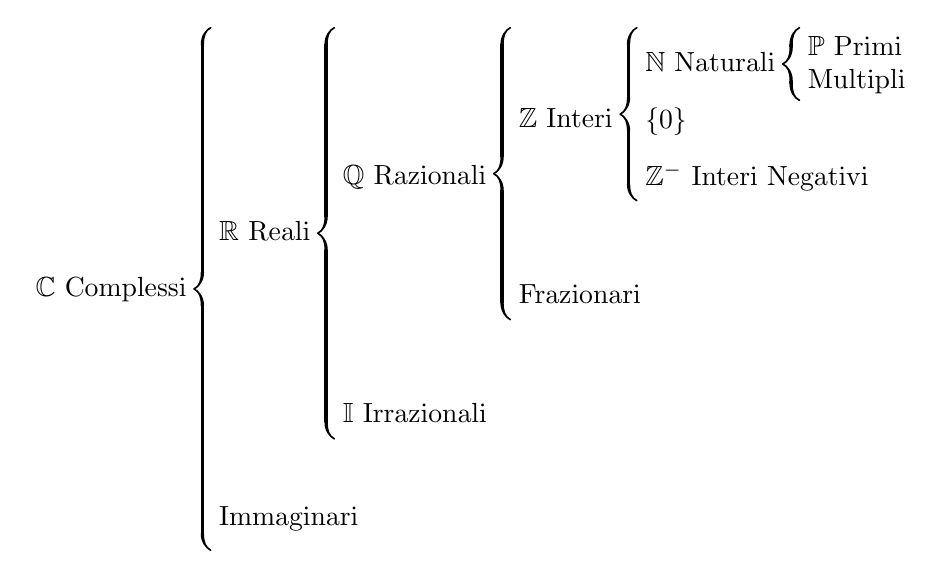
\begin{tikzpicture}[
node distance=1mm and 2mm,
every node/.style = {minimum height=6mm, text depth=0.3ex, inner sep=1mm, align=left},
        BC/.style = {decorate,
                     decoration={calligraphic brace, amplitude=6pt,
                     mirror},
                     very thick,
                     %pen colour={red}
                    },
                        ]
\node (n1)                      {$\mathbb{C}$ Complessi};
\node (n2)  [above right=of n1] {$\mathbb{R}$ Reali};
\node (n3)  [above right=of n2] {$\mathbb{Q}$ Razionali};
\node (n4)  [above right=of n3] {$\mathbb{Z}$ Interi};
\node (n5)  [above right=of n4] {$\mathbb{N}$ Naturali};
\node (n6)  [right=of n5]       {$\mathbb{P}$ Primi \\
                                 Multipli};
\path   let \p1 = (n1.east),
            \p2 = (n6.north west),
            \n1 = {veclen(\y2-\y1,\x2-\x1)} in
        coordinate[below=\y2-\y1 of n1.east -| n2.west] (c1);
\node (n7)  [above right=of c1 -| n1.east]
                                {Immaginari};
\node (n8)  [above right=7mm and 2mm of n7.north -| n2.east]
                                {$\mathbb{I}$ Irrazionali};
\node (n9)  [above right=9mm and 2mm of n8.north -| n3.east]
                                {Frazionari};
\node (n10) [right=of n4]       {$\{0\}$};
\node (n11) [right=of n3 -| n4.east]
                                {$\mathbb{Z}^-$ Interi Negativi};
%
\draw[BC]   (n6.north -| n2.west) -- (c1);
\draw[BC]   (n6.north -| n3.west) -- (n8.south west);
\draw[BC]   (n6.north -| n4.west) -- (n9.south west);
\draw[BC]   (n6.north -| n5.west) -- (n11.south west);
\draw[BC]   (n6.north west) -- (n6.south west);
    \end{tikzpicture}
\end{document}